\documentclass[10pt]{beamer}

\usepackage{Theme/BeamerTheme}
\usefonttheme[onlymath]{serif}
\usepackage{hyperref}
\hypersetup{pdfpagemode=FullScreen}
\usepackage{mathrsfs}
\usepackage{amsmath}
\usepackage{bm}
\usepackage{listings}
\usepackage{mathtools}
\usepackage{booktabs}
\usepackage{multirow}
\usepackage{ragged2e}
\justifying
\let\raggedright\justifying
\usepackage{tikz}
\usepackage{tkz-euclide}
\usetikzlibrary{shadows}
\usetikzlibrary{positioning}
\usetikzlibrary{circuits.ee.IEC}
\usetikzlibrary{decorations.pathmorphing}
\usetikzlibrary{shapes.symbols}
\usetkzobj{all}
\usepackage[framed,numbered]{matlab-prettifier}
\usepackage{pgfplots}
\usepgfplotslibrary{groupplots}
\usepgfplotslibrary{fillbetween}

\tikzset{
    text shadow/.code args={[#1]#2at#3(#4)#5}{
        \pgfkeysalso{/tikz/.cd,#1}%
        \foreach \angle in {0,5,...,359}{
                \node[#1,text=white] at ([shift={(\angle:.8pt)}] #4){#5};
        }
    }
}

\usepackage{tabu}
\usepackage{graphicx}
\usepackage{colortbl}
\usepackage{ifthen}
\usepackage{siunitx}
\ExplSyntaxOn
\cs_new_eq:NN \siunitx_table_collect_begin:Nn \__siunitx_table_collect_begin:Nn
\ExplSyntaxOff

\usepackage{soul}
\usepackage{keycommand}


\DeclareMathSizes{5}{5}{3}{3}

\newcommand{\pgfdefaultlinewidth}{0.75pt}
\newcommand{\risk}{\mathscr{R}}

\newkeycommand{\shadowtag}[align = center, background = white, x = 0, y = 0, color = black][1]{%
	\node at (\commandkey{x}, \commandkey{y}) [text shadow={[align=\commandkey{align}] at (\commandkey{x}, \commandkey{y}) {#1}}, align = \commandkey{align}] {\textcolor{\commandkey{color}}{#1}};
}

\newcommand{\code}[1]{
    \texttt{\textcolor[rgb]{0.00,0.00,1.00}{#1}}
}

\makeatletter
\lstnewenvironment{bash}[1][]{%
  \lstset{%
    #1,
    style = Matlab-editor,
    numbers=left,
    numberstyle = \scriptsize,
    basicstyle = \ttfamily\footnotesize,
    firstnumber=auto,
  }%
  \csname\@lst @SetFirstNumber\endcsname
}{%
  \csname \@lst @SaveFirstNumber\endcsname
}
\makeatother

\begin{document}

% Cover
% \maketitle
\begin{frame}[plain, noframenumbering]\label{Title}
    \vfill
    \centering
    \usebeamerfont{title}\Huge
    Monthly Report\\
    \begin{tikzpicture}\draw[mLightBrown, line width = 1pt] (0, 0) -- (\textwidth, 0);\end{tikzpicture}\vspace{15pt}\\
    \begin{minipage}[m]{3cm}
        \Bold \small Zhang Qi
    \end{minipage}\hspace{-15pt}
    \begin{minipage}[m]{1.5cm}
        \centering
        
\includegraphics[height=0.8cm]{Logos/HUSTLogoWithoutSubline.pdf}
    \end{minipage}
    \begin{minipage}[m]{0.55\textwidth}
        \Normal \scriptsize School of Automation,\\Huazhong University of Science and Technology,\\Wuhan, China.
    \end{minipage}
    \vfill
    \centering
    \usebeamerfont{date}\usebeamercolor[fg]{date}\today
\end{frame}

% Outlines
\begin{frame}[noframenumbering]{Outlines}\label{Outlines}
    \setcounter{tocdepth}{1}
    \tableofcontents % [pausesections]
\end{frame}

% Main Body
\section{Multiple Models for Risk Assessment}
\begin{frame}{Seven Factors about the Risk}
\vspace{10pt}\hspace{-30pt}
\begin{minipage}{1.12\textwidth}
    \begin{itemize}[<+->]
      \item \textbf{Attack Strategy} refers to the atom attack which is launched by an attacker to achieve his destructive purpose.
      \item \textbf{System Function} refers to the function of control system.
      \item \textbf{Security Strategy} is a kind of defense strategy which can prevent attack strategy.
      \item \textbf{Recover Strategy} is a kind of defense strategy which can recover the failed system function.
      \item \textbf{Hazardous Incident} refers to the unexpected incident which will cause monetary loss of ICSs.
      \item \textbf{Production Process} refers a manufacturing step which is a part of in a production chain.
      \item \textbf{Monetary Loss} is the sum of the loss caused by malicious attacks, the loss of production process shutdown, and the enforcement cost of defense strategy.
    \end{itemize}
\end{minipage}
\end{frame}

\begin{frame}{The relationships amongst these seven factors}
\vspace{10pt}\hspace{-35pt}
\begin{minipage}{0.6\textwidth}
\begin{itemize}[<+->]
  \item The attack strategy can invalidate the system function.
  \item The failure of the system function can lead to hazardous incident and product process shutdown.
  \item The occurrence of these two unexpected events will both cause the monetary loss of ICSs.
  \item The security strategy will prevent the enforcement of attack strategy, but its side effect is that it may invalidate the system function.
  \item The recover strategy has ability of recovering the failed system function, and it has the enforcement cost.
\end{itemize}
\end{minipage}
\hspace{5pt}
\begin{minipage}{0.38\textwidth}
    \scalebox{0.63}{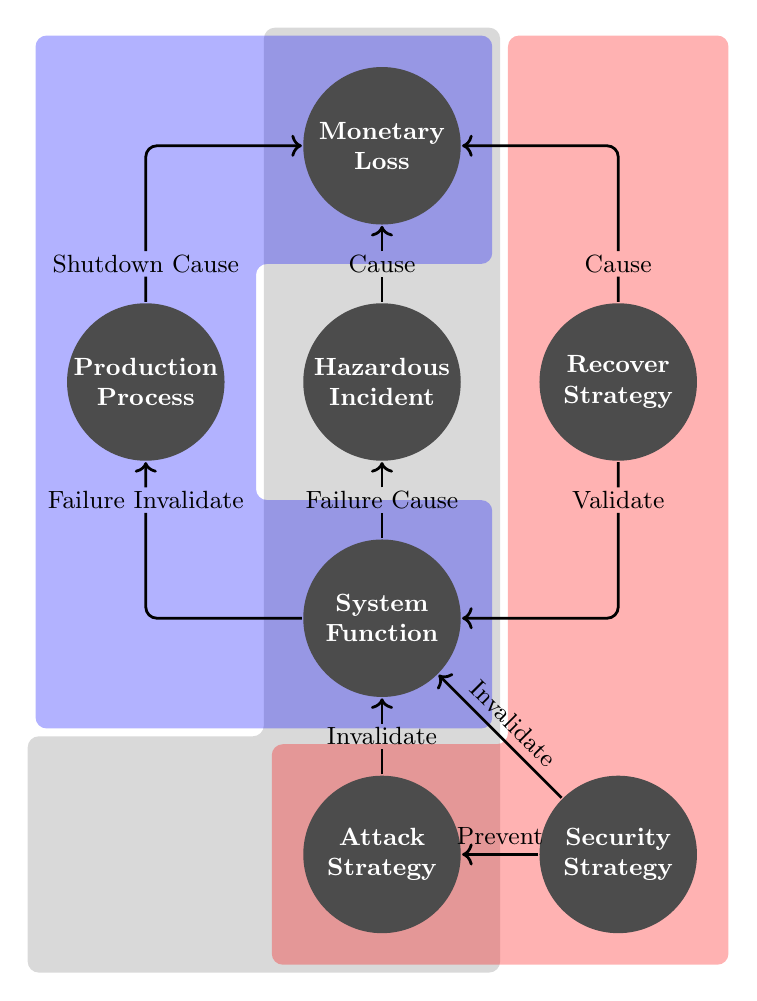
\begin{tikzpicture}[line width = 1pt,
                    factor/.style = {circle, fill = black!70, text = white, font = \bf, inner sep = 0pt, align = center, minimum size = 2cm},
                    tag/.style = {align = center, inner sep = 1pt},
                    model/.style = {rounded corners, opacity= 0.3},
                    arrow/.style = {->, rounded corners}]

\small
\fill[gray, model] (-0.5, 0.5) -- (-0.5, 3.5) -- (2.5, 3.5) -- (2.5, 12.5) -- (5.5,12.5) -- (5.5, 0.5) -- cycle;
\fill[blue, model] (-0.4, 12.4) -- (5.4, 12.4) -- (5.4, 9.5) -- (2.4, 9.5) -- (2.4, 6.5) -- (5.4, 6.5) -- (5.4, 3.6) -- (-0.4, 3.6) -- cycle;
\fill[red, model] (5.6,3.4) -- (5.6, 12.4) -- (8.4,12.4) -- (8.4, 0.6) -- (2.6, 0.6) -- (2.6, 3.4) -- cycle;


\shadowtag[x = 1, y = 2.2]{\bf Multi-level}
\shadowtag[x = 1, y = 1.8]{\bf Bayesian Network}
\shadowtag[x = 1, y = 4.2, color = blue]{\bf Process Model}
\shadowtag[x = 7, y = 4.4, color = red]{\bf Attack-Defense}
\shadowtag[x = 7, y = 4.0, color = red]{\bf Strategies Models}


\node[tag] (AS2SF) at (4, 3.5) {Invalidate};
\node[tag] (SF2HI) at (4, 6.5) {Failure Cause};
\node[tag] (SF2PP) at (1, 6.5) {Failure Invalidate};
\node[tag] (RS2SF) at (7, 6.5) {Validate};

\node[tag] (PP2ML) at (1, 9.5) {Shutdown Cause};
\node[tag] (HI2ML) at (4, 9.5) {Cause};
\node[tag] (RS2ML) at (7, 9.5) {Cause};

\node[factor] (ML) at (4, 11) {Monetary\\Loss};
\node[factor] (HI) at (4,  8) {Hazardous\\Incident};
\node[factor] (SF) at (4,  5) {System\\Function};
\node[factor] (AS) at (4,  2) {Attack\\Strategy};
\node[factor] (PP) at (1,  8) {Production\\Process};
\node[factor] (RS) at (7,  8) {Recover\\Strategy};
\node[factor] (SS) at (7,  2) {Security\\Strategy};

\draw[arrow] (AS) -- (AS2SF) -- (SF);
\draw[arrow] (SF) -- (SF2HI) -- (HI);
\draw[arrow] (HI) -- (HI2ML) -- (ML);
\draw[arrow] (SF) -| (SF2PP) -- (PP);
\draw[arrow] (PP) -- (PP2ML) |- (ML);

\draw[arrow] (RS) -- (RS2ML) |- (ML);
\draw[arrow] (RS) -- (RS2SF) |- (SF);

\draw[arrow] (SS) -- (SF) node[midway, sloped, above] {Invalidate};
\draw[arrow] (SS) -- (AS) node[midway, sloped, above] {Prevent};
\end{tikzpicture}}
\end{minipage}
\end{frame}

\begin{frame}{Multiple Models of Risk Assessment for ICSs}
The following three models are used to described the relationships amongst these seven factors.

\begin{itemize}[<+->]
  \item The \textbf{multi-level Bayesian network}, involves attack strategy, system function, hazardous incident, and monetary loss. This model uses Bayesian network to describe the causal relationship of these four factors and it can be used to assess the risk caused by the malicious attacks.
  \item The \textbf{process model} involves system functions, production process, and monetary loss. It can be used to calculate the risk cause by the degradation of control system.
  \item The \textbf{attack-defense strategies models}, include attack strategy model, security strategy model, and recover strategy model. These three models contain the relationships amongst these three kinds of strategies and system functions, and they can be used to quantify the cost and benefit of attack-defense strategies.
\end{itemize}
\end{frame}

\begin{frame}{Chemical Reactor Control System}
    \resizebox{\textwidth}{!}{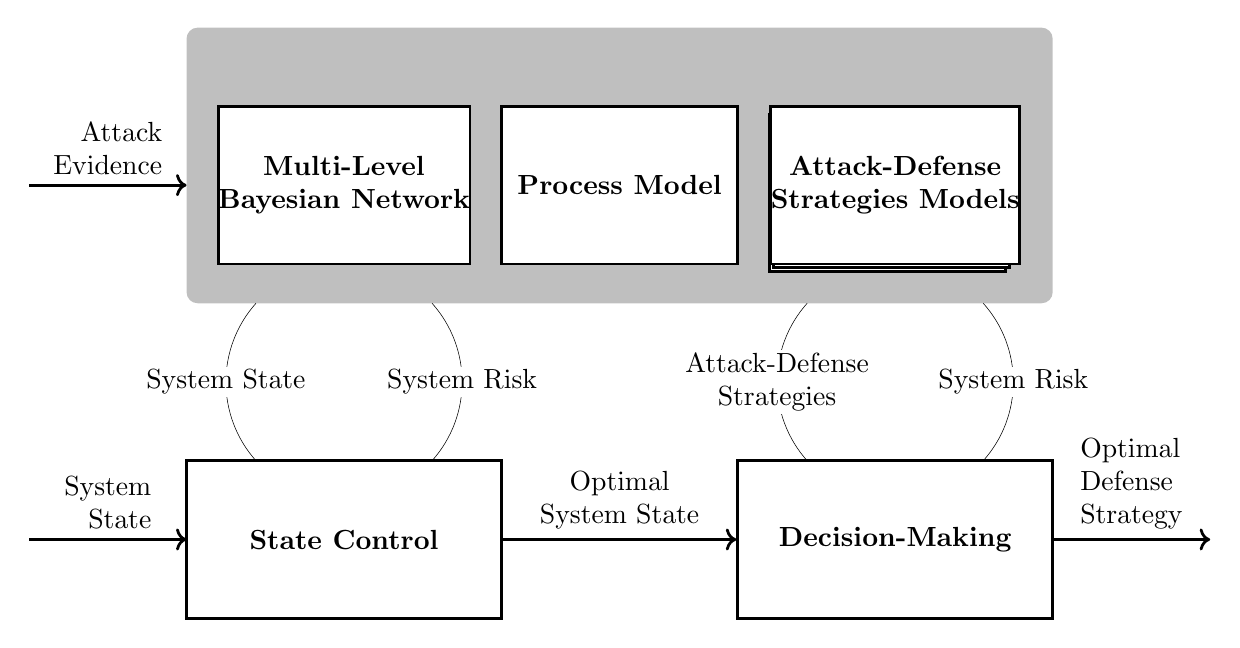
\begin{tikzpicture}[line width = 1pt,
                    model/.style = {rectangle, draw, fill = white, text = black, font = \bf, inner sep = 0pt, align = center, minimum height = 2cm, minimum width = 3cm},
                    block/.style = {rectangle, draw, fill = white, text = black, font = \bf, inner sep = 0pt, align = center, minimum height = 2cm, minimum width = 4cm},
                    tag/.style = {align = center, inner sep = 1pt, fill = white}]

\fill[rounded corners, gray, opacity = 0.5] (1, 6) rectangle (12,9.5);

\node[model] at (  3, 7.5) {Multi-Level\\Bayesian Network};
\node[model] at (6.5, 7.5) {Process Model};
\foreach \i in {2, 1}{
	\node[model] at (10 - 0.05 * \i, 7.5 - 0.05 * \i) {};	
}
\node[model] at (10, 7.5) {Attack-Defense\\Strategies Models};
\shadowtag[x = 6.5, y = 9]{\Large Multiple Models for ICSs};

\node[block] (SC) at ( 3, 3) {State Control};
\node[block] (DM) at (10, 3) {Decision-Making};

\draw[->] (-1, 3) -- (1,3) node [align = right, above, minimum width = 2cm, midway] {System\\State};
\draw[->] (-1, 7.5) -- (1, 7.5) node [align = right, above, minimum width = 2cm, midway] {Attack\\Evidence};
\draw[->] (SC) -- (DM) node[midway, align = center, above] {Optimal\\System State};
\draw[->] (12,3) -- (14, 3) node[align = left, above, midway] {Optimal\\Defense\\Strategy};

\begin{scope}
	\draw[name path=rectangle, draw = none] (1,4) rectangle (5,6);
	\draw[name path=circle, draw = none] (3, 5) circle (1.5);
	\tkzDefPoint(3,5){O}
	\draw [name intersections={of=rectangle and circle, by={a,b,c,d}}] (b) circle (0pt);
	
	\tikzset{compass style/.append style={<-, line width= 1pt}}
	\tkzDrawArc[color=black](O,b)(c)
	\tkzDrawArc[color=black](O,d)(a)
\end{scope}

\begin{scope}
\draw[name path=rectangle, draw = none] (8,4) rectangle (12,6);
\draw[name path=circle, draw = none] (10, 5) circle (1.5);
\tkzDefPoint(10,5){O}
\draw [name intersections={of=rectangle and circle, by={a,b,c,d}}] (b) circle (0pt);

\tikzset{compass style/.append style={<-, line width= 1pt}}
\tkzDrawArc[color=black](O,b)(c)
\tkzDrawArc[color=black](O,d)(a)
\end{scope}

\node[tag] at (1.5, 5) {System State};
\node[tag] at (4.5, 5) {System Risk};
\node[tag] at (8.5, 5) {Attack-Defense\\Strategies};
\node[tag] at (11.5, 5) {System Risk};
\end{tikzpicture}}
\end{frame}

\section{Simulation}
\subsection{A Failed Attempt}
\begin{frame}{A Failed Attempt --- C++ Version}
    I had implemented the class \code{Node} and the class \code{BayesianNetwork} with C++ language.

    The inference of Bayesian network is provided by \code{dlib}, which is a C++ library. But the computation time of the Bayesian network inference is 30 times slower than that of the implementation by Matlab.\vspace{5pt}

    \begin{center}
    \tabulinesep =1.5mm
    \begin{tabu}to 0.8\textwidth{X[l]X[r]}
        \tabucline[1pt]{-}
        Runtime Environment  & Computation Time(ms)\\
        \hline
        C++ in Debug Mode    & 40,000\\
        C++ in Release Mode  & 3,600\\
        Matlab               & 90\\
        \tabucline[1pt]{-}
    \end{tabu}\vspace{5pt}
    \end{center}

    The Matlab has optimized the algorithm for a large amount of computation.
\end{frame}

\subsection{Common Simulation Platform}
\begin{frame}{Common Classes}
    For the simulation, the following common classes are designed:

    class \code{Node}, \pause 
    class \code{Evidence}, \pause 
    class \code{BayesianNetwork}, \pause 
    class \code{Product}, \pause 
    class \code{Process}, \pause 
    class \code{ProductionModel}, \pause 
    class \code{SystemState}, \pause 
    class \code{RiskModel}, \pause 
    class \code{Strategies.Security}, \pause 
    class \code{Strategies.Recover}, and \pause 
    class \code{DecisionMaker}.

    \pause
    The relationship amongst these classes are shown as follows.

    \resizebox{\textwidth}{!}{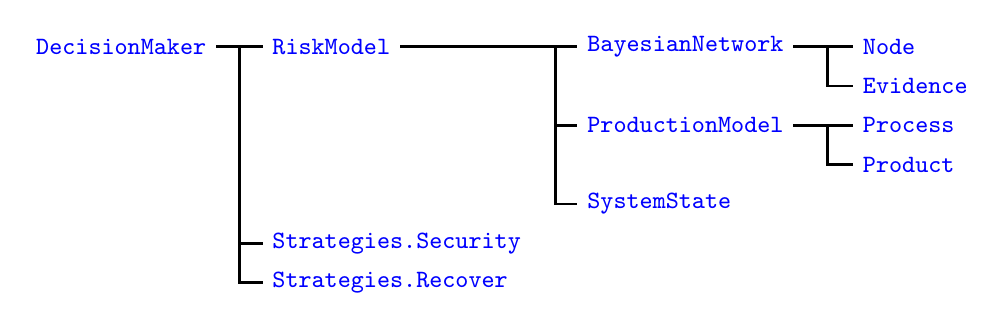
\begin{tikzpicture}[line width = 1pt]

\small

\node[anchor = west] (DM) at ( 0, 9.0) {\code{DecisionMaker}};
\node[anchor = west] (RM) at ( 3, 9.0) {\code{RiskModel}};
\node[anchor = west] (SS) at ( 3, 6.5) {\code{Strategies.Security}};
\node[anchor = west] (SR) at ( 3, 6.0) {\code{Strategies.Recover}};
\node[anchor = west] (BN) at ( 7, 9.0) {\code{BayesianNetwork}};
\node[anchor = west] (PM) at ( 7, 8.0) {\code{ProductionModel}};
\node[anchor = west] (ST) at ( 7, 7.0) {\code{SystemState}};

\node[anchor = west] (ND) at (10.5, 9.0) {\code{Node}};
\node[anchor = west] (EV) at (10.5, 8.5) {\code{Evidence}};
\node[anchor = west] (PR) at (10.5, 8.0) {\code{Process}};
\node[anchor = west] (PD) at (10.5, 7.5) {\code{Product}};

\draw (DM) -- (RM)
      (DM) -- ++(0:1.5cm) |- (SS)
      (DM) -- ++(0:1.5cm) |- (SR);

\draw (RM) -- (BN)
      (RM) -- ++(0:2.85cm) |- (PM)
      (RM) -- ++(0:2.85cm) |- (ST);   
      
\draw (BN) -- (ND)
      (BN) -- ++(0:1.8cm) |- (EV);
      
\draw (PM) -- (PR)
      (PM) -- ++(0:1.8cm) |- (PD);      

\end{tikzpicture} }
\end{frame}

\begin{frame}[fragile]
\frametitle{How to Use?}
The following example is used to introduce how to use the class \code{Node} and class \code{BayesianNetwork} to model and inference the Bayesian network.\vspace{10pt}

\pause
\begin{minipage}[t]{0.4\textwidth}
    The Bayesian network is shown as follows.\vspace{10pt}
    \centering
    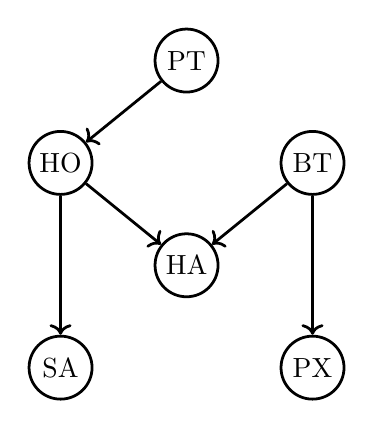
\begin{tikzpicture}[line width = 1pt,
                    x = 1.6cm,
                    y = 1.3cm,
                    node/.style = {circle, draw, inner sep = 0pt, minimum size = 0.8cm}]

    % \grid{0}{15}{0}{13}
    \node[node] (PT) at (1,3) {PT};
    \node[node] (HO) at (0,2) {HO};
    \node[node] (BT) at (2,2) {BT};
    \node[node] (SA) at (0,0) {SA};
    \node[node] (PX) at (2,0) {PX};
    \node[node] (HA) at (1,1) {HA};

    \foreach \i/\j in {PT/HO,
                       HO/HA,
                       BT/HA,
                       HO/SA,
                       BT/PX}
    {
        \draw[->] (\i) -- (\j);
    }
\end{tikzpicture}
\end{minipage}\hspace{10pt}\pause
\begin{minipage}[t]{0.55\textwidth}
    The meanings of nodes are shown as follows.\vspace{10pt}

    \tabulinesep =1.5mm
    \begin{tabu}{@{}X[-1,c]X[-1]@{}}
      \tabucline[1pt]{-}
      Symbol & Meaning\\
      \hline
      PT & Qiqi goes to the Party.\\
      HO & Qiqi has a Hangover.\\
      BT & Qiqi has a Brain Tumor.\\
      HA & Qiqi has a Headache.\\
      SA & Qiqi has an Alcohol Smell.\\
      PX & Qiqi has a Pos Xray.\\
      \tabucline[1pt]{-}
    \end{tabu}
\end{minipage}
\end{frame}

\begin{frame}[fragile]
\frametitle{How to Use?}
Step 1, create the nodes of Bayesian network.
\begin{bash}[name=BayesianNetwork]
PT = Classes.Node('Party');
HO = Classes.Node('Hangover');
BT = Classes.Node('Brain Tumor');
HA = Classes.Node('Headache');
SA = Classes.Node('Smell Alcohol');
PX = Classes.Node('Pos Xray');
\end{bash}

Step 2, set the conditional probabilities of nodes.
\begin{bash}[name=BayesianNetwork]
PT.AddAllParents(... Has no parent node
    0.200);

BT.AddAllParents(... Has no parent node
    0.001);
\end{bash}
\end{frame}

\begin{frame}[fragile]
\frametitle{How to Use?}
\begin{bash}[name=BayesianNetwork]
HO.AddAllParents(PT, ...
    0.000, ...    F
    0.700);  %    T

SA.AddAllParents(HO, ...
    0.100, ...    F
    0.800);  %    T

PX.AddAllParents(BT, ...
    0.010, ...    F
    0.980);  %    T

HA.AddAllParents(HO, BT, ...
    0.020, ...    F   F
    0.900, ...    F   T
    0.700, ...    T   F
    0.990);  %    T   T
\end{bash}
\end{frame}

\begin{frame}[fragile]
\frametitle{How to Use?}
Step 3, create the Bayesian network.
\begin{bash}[name=BayesianNetwork]
BayesianNetwork = Classes.BayesianNetwork();
\end{bash}

Step 4, add the nodes into the Bayesian network.
\begin{bash}[name=BayesianNetwork]
BayesianNetwork.AddNodes(PT, BT, HO, SA, PX, HA);
\end{bash}

Step 5, initialize the Bayesian network.
\begin{bash}[name=BayesianNetwork]
BayesianNetwork.Initialize();
\end{bash}

Step 6, infer the Bayesian network.
\begin{bash}[name=BayesianNetwork]
BayesianNetwork.Inference();
BayesianNetwork.Display(HA);
\end{bash}
\end{frame}

\begin{frame}[fragile]
\frametitle{How to Use?}
\textbf{Question:} if Qiqi has a Pos Xray (PX), what's the probability that Qiqi has a Brain Tumor (BT)?

The Matlab codes are shown as follows.
\begin{bash}[name=BayesianNetwork]
% Remove all the evidences in the Bayesian network.
BayesianNetwork.RemoveEvidences();

% Add the evidence PX into the evidence list.
BayesianNetwork.AddEvidences(PX);

% Infer the Bayesian network with the evidences.
BayesianNetwork.Inference();

% Show the probability of the node BT.
BayesianNetwork.Display(BT);
\end{bash}

The output of the program is shown as follows.
\begin{bash}
P(+Brain Tumor|+Pos Xray) = 0.089335
\end{bash}

\end{frame}

\subsection{Simulation Object}
\begin{frame}{Chemical Reactor Control System}
    \hspace{-10pt}\resizebox{\textwidth}{!}{\definecolor{textcolor}{rgb}{0, 0, 0}

\tikzset{circuit declare symbol = ac source}
\tikzset{set ac source graphic = ac source IEC graphic}
\tikzset
{
    ac source IEC graphic/.style=
    {
        transform shape,
        circuit symbol lines,
        circuit symbol size = width 3 height 3,
        shape=generic circle IEC,
        /pgf/generic circle IEC/before background=
        {
            \pgfpathmoveto{\pgfpoint{-0.8pt}{0pt}}
            \pgfpathsine{\pgfpoint{0.4pt}{0.4pt}}
            \pgfpathcosine{\pgfpoint{0.4pt}{-0.4pt}}
            \pgfpathsine{\pgfpoint{0.4pt}{-0.4pt}}
            \pgfpathcosine{\pgfpoint{0.4pt}{0.4pt}}
            \pgfusepathqstroke
        }
    }
}

\tikzset{
	text shadow/.code args={[#1]#2at#3(#4)#5}{
		\pgfkeysalso{/tikz/.cd,#1}%
		\foreach \angle in {0,5,...,359}{
			\node[#1,text=white] at ([shift={(\angle:.8pt)}] #4){#5};
		}
	}
}

\newkeycommand{\reactor}[x = 0, y = 0, width = 2cm, height = 3cm, archeight = 1cm, name = reactor, level = -1cm, textpos = 0cm][1]{
    \draw
    (\commandkey{x} - 0.5*\commandkey{width}, \commandkey{y} - 0.5*\commandkey{height} + \commandkey{archeight}) to[out = -90, in = 180]
    (\commandkey{x}, \commandkey{y} - 0.5*\commandkey{height}) to[out = 0, in = -90]
    (\commandkey{x} + 0.5*\commandkey{width}, \commandkey{y} - 0.5*\commandkey{height} + \commandkey{archeight}) --
    (\commandkey{x} + 0.5*\commandkey{width}, \commandkey{y} + 0.5*\commandkey{height} - \commandkey{archeight}) to[out = 90, in = 0]
    (\commandkey{x}, \commandkey{y} + 0.5*\commandkey{height}) to[out = 180, in = 90]
    (\commandkey{x} - 0.5*\commandkey{width}, \commandkey{y} + 0.5*\commandkey{height} - \commandkey{archeight}) --
    cycle;
    \node[rectangle, minimum width = \commandkey{width}, minimum height = \commandkey{height}] (\commandkey{name}) at (\commandkey{x}, \commandkey{y}){};

    \node[align = center] at (\commandkey{x}, \commandkey{y} - 0.5*\commandkey{height} + 0.5*\commandkey{archeight} + \commandkey{textpos}) {#1};

    \begin{scope}
      \clip (\commandkey{x} - 0.5*\commandkey{width}, \commandkey{y} - 0.5*\commandkey{height} + \commandkey{archeight}) to[out = -90, in = 180]
        (\commandkey{x}, \commandkey{y} - 0.5*\commandkey{height}) to[out = 0, in = -90]
        (\commandkey{x} + 0.5*\commandkey{width}, \commandkey{y} - 0.5*\commandkey{height} + \commandkey{archeight}) --
        (\commandkey{x} + 0.5*\commandkey{width}, \commandkey{y} + 0.5*\commandkey{height} - \commandkey{archeight}) to[out = 90, in = 0]
        (\commandkey{x}, \commandkey{y} + 0.5*\commandkey{height}) to[out = 180, in = 90]
        (\commandkey{x} - 0.5*\commandkey{width}, \commandkey{y} + 0.5*\commandkey{height} - \commandkey{archeight}) --
        cycle;
      \draw[blue, decorate, decoration={snake}]
      (\commandkey{x} - \commandkey{width}, \commandkey{y} - 0.5*\commandkey{height} + \commandkey{level}) --
      (\commandkey{x} + \commandkey{width}, \commandkey{y} - 0.5*\commandkey{height} + \commandkey{level});
    \end{scope}
}

\newkeycommand{\bus}[x = 0, y = 0, width = 0.5cm, length = 5cm, inner sep = 2pt, name = bus][1]{
    \draw
    (\commandkey{x} - 0.5*\commandkey{length}, \commandkey{y} + 0.5*\commandkey{width}) --
    (\commandkey{x} + 0.5*\commandkey{length}, \commandkey{y} + 0.5*\commandkey{width})
    to [out = 0, in = 0]
    (\commandkey{x} + 0.5*\commandkey{length}, \commandkey{y} - 0.5*\commandkey{width}) --
    (\commandkey{x} - 0.5*\commandkey{length}, \commandkey{y} - 0.5*\commandkey{width})
    to [out = 180, in = 180] cycle;

    \draw
    (\commandkey{x} + 0.5*\commandkey{length}, \commandkey{y} + 0.5*\commandkey{width} - \commandkey{inner sep}) to [out = 0, in = 0]
    (\commandkey{x} + 0.5*\commandkey{length}, \commandkey{y} - 0.5*\commandkey{width} + \commandkey{inner sep}) to [out = 180, in = 180] cycle;

    \node[rectangle, minimum width = \commandkey{length}, minimum height = \commandkey{width}] (\commandkey{name}) at (\commandkey{x}, \commandkey{y}) {#1};
}

\newkeycommand{\computer}[x = 0cm, y = 0cm, width = 2cm, height = 2cm, name = computer][1]{
    \node at (\commandkey{x}, \commandkey{y}) {
\includegraphics[width=\commandkey{width}]{Figures/Material/Computer.pdf}};
    \node[rectangle, minimum width = 0.82*\commandkey{width}, minimum height = 0.82*\commandkey{height}] (\commandkey{name}) at (\commandkey{x}, \commandkey{y}){};
    \node at (\commandkey{x} - 0.5*\commandkey{width}, \commandkey{y} + 0.5*\commandkey{height}) [text shadow={[align=left, anchor = north west, inner sep = 0pt] at (\commandkey{x} - 0.5*\commandkey{width}, \commandkey{y} + 0.5*\commandkey{height}) {\parbox{\commandkey{width}}{\raggedright #1}}}, align = left, anchor = north west, inner sep = 0pt] {\textcolor{black}{\parbox{\commandkey{width}}{\raggedright \textcolor{textcolor}{#1}}}};
}

\newkeycommand{\server}[x = 0cm, y = 0cm, width = 1.35cm, height = 2cm, name = server][1]{
    \node at (\commandkey{x}, \commandkey{y}) {
\includegraphics[width=\commandkey{width}]{Figures/Material/Server.pdf}};
    \node[rectangle, minimum width = 1.16*\commandkey{width}, minimum height = 0.76*\commandkey{height}] (\commandkey{name}) at (\commandkey{x}, \commandkey{y}){};
    \node at (\commandkey{x} - 0.5*\commandkey{width}, \commandkey{y} + 0.5*\commandkey{height}) [text shadow={[align=left, anchor = north west, inner sep = 0pt] at (\commandkey{x} - 0.5*\commandkey{width}, \commandkey{y} + 0.5*\commandkey{height}) {\parbox{\commandkey{width}}{\raggedright #1}}}, align = left, anchor = north west, inner sep = 0pt] {\textcolor{black}{\parbox{\commandkey{width}}{\raggedright \textcolor{textcolor}{#1}}}};
}

\newkeycommand{\plc}[x = 0cm, y = 0cm, width = 1.8cm, height = 2cm, name = plc][1]{
    \node at (\commandkey{x}, \commandkey{y}) {
\includegraphics[width=\commandkey{width}]{Figures/Material/PLC.pdf}};
    \node[rectangle, minimum width = 0.76*\commandkey{width}, minimum height = 0.76*\commandkey{height}] (\commandkey{name}) at (\commandkey{x}, \commandkey{y}){};
    \node at (\commandkey{x}, \commandkey{y}) [text shadow={[align=center, inner sep = 0pt] at (\commandkey{x}, \commandkey{y}) {\parbox{\commandkey{width}}{\centering #1}}}, align = center, inner sep = 0pt] {\textcolor{black}{\parbox{\commandkey{width}}{\centering \textcolor{textcolor}{#1}}}};
}

\newkeycommand{\gateway}[x = 0cm, y = 0cm, width = 1.8cm, height = 1.5cm, name = gateway][1]{
    \node at (\commandkey{x}, \commandkey{y}) {
\includegraphics[width=\commandkey{width}]{Figures/Material/Gateway.pdf}};
    \node[rectangle, minimum width = \commandkey{width}, minimum height = 0.74*\commandkey{height}] (\commandkey{name}) at (\commandkey{x}, \commandkey{y} - 0.08cm){};
    \node at (\commandkey{x}, \commandkey{y}) [text shadow={[align=center, inner sep = 0pt] at (\commandkey{x}, \commandkey{y}) {\parbox{\commandkey{width}}{\centering #1}}}, align = center, inner sep = 0pt] {\textcolor{black}{\parbox{\commandkey{width}}{\centering \textcolor{textcolor}{#1}}}};
}

\newkeycommand{\valve}[x = 0cm, y = 0cm, width = 0.6cm, height = 0.4cm, name = valve][1]{
    \node[rectangle, minimum width = \commandkey{width}, minimum height = 2.3*\commandkey{height}, inner sep = 0pt] (\commandkey{name}) at (\commandkey{x}, \commandkey{y}){};
    \draw (\commandkey{x} + 0.5*\commandkey{width}, \commandkey{y} + 0.5*\commandkey{height}) --
          (\commandkey{x} + 0.5*\commandkey{width}, \commandkey{y} - 0.5*\commandkey{height}) --
          (\commandkey{x} - 0.5*\commandkey{width}, \commandkey{y} + 0.5*\commandkey{height}) --
          (\commandkey{x} - 0.5*\commandkey{width}, \commandkey{y} - 0.5*\commandkey{height}) -- cycle;
    \draw (\commandkey{x}, \commandkey{y}) --
          (\commandkey{x}, \commandkey{y} + 0.85*\commandkey{height}) --
          (\commandkey{x} - 0.5*\commandkey{width}, \commandkey{y} + 0.85*\commandkey{height})
          to [out = 45, in = 135]
          (\commandkey{x} + 0.5*\commandkey{width}, \commandkey{y} + 0.85*\commandkey{height}) --
          (\commandkey{x}, \commandkey{y} + 0.85*\commandkey{height});
    \node[below = 5pt] at (\commandkey{x}, \commandkey{y}) {#1};
}

\newkeycommand{\switch}[x = 0cm, y = 0cm, width = 0.5cm, name = switch][1]{
    \node[rectangle, minimum width = \commandkey{width}, minimum height = 0.5774*\commandkey{width}, inner sep = 0pt] (\commandkey{name}) at (\commandkey{x}, \commandkey{y}) {};
    \draw (\commandkey{x} - 0.5*\commandkey{width}, \commandkey{y}) -- ++(30:\commandkey{width});
    \node[draw, circle, minimum size = 1pt, fill = white, inner sep = 0pt] at (\commandkey{x} - 0.5*\commandkey{width}, \commandkey{y}) {};
    \node[below = 0pt] at (\commandkey{x}, \commandkey{y}) {#1};
}

\newkeycommand{\motor}[x = 0cm, y = 0cm, width = 0.7cm, name = motor][1]{
    \node[draw, circle, minimum size = \commandkey{width}, inner sep = 0pt] (\commandkey{name}) at (\commandkey{x}, \commandkey{y}) {#1};
}

\newkeycommand{\sensor}[x = 0cm, y = 0cm, width = 0.18cm, height = 0.5cm, name = sensor][1]{
    \node[rectangle, inner sep = 0pt, minimum width = \commandkey{width}, minimum height = \commandkey{height}, fill = black] (\commandkey{name}) at (\commandkey{x}, \commandkey{y}) {};
    \node[below = 0.5*\commandkey{height}] at (\commandkey{x}, \commandkey{y}) {#1};
}

\newkeycommand{\omission}[x = 0cm, y = 0cm, angle = 0, length = 0.4cm, name = omission]{
    \begin{scope}
    \clip[rotate around={\commandkey{angle}:(\commandkey{x}, \commandkey{y})}] (\commandkey{x} - 0.45*\commandkey{length} , \commandkey{y} - 0.45*\commandkey{length} ) rectangle (\commandkey{x} + 0.45*\commandkey{length}  , \commandkey{y} + 0.45*\commandkey{length} );
    \foreach \x/\c in {1pt/white,
                       2pt/black,
                       3pt/white,
                       4pt/black,
                       5pt/white}{
    \draw[line width = 1pt, draw = \c] (\commandkey{x}, \commandkey{y} - 3pt + \x) to[out = 120 + \commandkey{angle}, in = 60 + \commandkey{angle}] ++(180 + \commandkey{angle}:0.5*\commandkey{length})
        (\commandkey{x}, \commandkey{y} - 3pt + \x) to[out = -60 + \commandkey{angle}, in = -120 + \commandkey{angle}] ++(\commandkey{angle}:0.5*\commandkey{length});

    }
    \end{scope}
}

\newkeycommand{\coverpipe}[x = 0cm, y = 0cm, length = 1cm, name = coverpipe]{
    \draw[dashed, line width = 4pt, draw = white, dash pattern = on 2pt off 3pt] (\commandkey{x} - 0.5*\commandkey{length}, \commandkey{y}) -- ++ (0:\commandkey{length});
    \draw (\commandkey{x} - 0.5*\commandkey{length}, \commandkey{y} + 3pt) -- (\commandkey{x} - 0.5*\commandkey{length}, \commandkey{y} - 3pt);
    \draw (\commandkey{x} + 0.5*\commandkey{length}, \commandkey{y} + 3pt) -- (\commandkey{x} + 0.5*\commandkey{length}, \commandkey{y} - 3pt);

    \draw[white] (\commandkey{x} - 0.5*\commandkey{length} - 1pt, \commandkey{y} + 3pt) -- (\commandkey{x} - 0.5*\commandkey{length} - 1pt, \commandkey{y} - 3pt);
    \draw[white] (\commandkey{x} + 0.5*\commandkey{length} + 1pt, \commandkey{y} + 3pt) -- (\commandkey{x} + 0.5*\commandkey{length} + 1pt, \commandkey{y} - 3pt);
}

\newkeycommand{\blender}[x = 0cm, y = 0cm, length = 2cm, name = blender][1]{
    \coordinate (\commandkey{name}) at (\commandkey{x}, \commandkey{y});
    \fill (\commandkey{x}, \commandkey{y})
    to [out = 30, in = 150] ++ (0:0.5*\commandkey{length})
    to [out = -150, in = -30] (\commandkey{x}, \commandkey{y})
    to [out = 150, in = 30] ++ (180:0.5*\commandkey{length})
    to [out = -30, in = -150] (\commandkey{x}, \commandkey{y});
    \node[anchor = north] at (\commandkey{name}) {#1};
}

\newkeycommand{\internet}[x = 0cm, y = 0cm, width = 2cm, name = internet][1]{
    \node[draw, cloud, minimum width = \commandkey{width}, minimum height = 1.5cm, inner sep = 0pt] (\commandkey{name}) at (\commandkey{x}, \commandkey{y}) {#1};
}

\newkeycommand{\heater}[x = 0cm, y = 0cm, width = 0.5cm, coverpos = 0.5cm, length = 2cm, name = heater][1]{
    \node[rectangle, minimum width = \commandkey{width}, minimum height = 0.5774*\commandkey{width}, inner sep = 0pt] (\commandkey{name}S) at (\commandkey{x}, \commandkey{y}) {};
    \draw (\commandkey{x} - 0.5*\commandkey{width}, \commandkey{y}) -- ++(30:\commandkey{width});
    \node[draw, circle, minimum size = 1pt, fill = white, inner sep = 0pt] at (\commandkey{x} - 0.5*\commandkey{width}, \commandkey{y}) {};
    \node[below = 0pt] at (\commandkey{x}, \commandkey{y}) {#1};

    \draw[line width = 1pt, draw = white, double=black, double distance = 1pt]
    (\commandkey{name}S) --
    ++(0:\commandkey{length}) to[resistor ={minimum width = 0.8cm, minimum height = 0.1cm}]
    ++(-90:1cm) --
    ++(180:1cm + \commandkey{length}) to[ac source = {rotate = 90, minimum size = 0.7cm}]
    ++(90:1cm) -- (\commandkey{name}S);
}

\linespread{0.9}

\begin{tikzpicture}[circuit ee IEC,
                    set resistor graphic=var resistor IEC graphic,
                    line width = 1pt,
                    x = 1cm,
                    y = 1cm,
                    pipe/.style = {line width = 1pt, draw = white, double=black, double distance = 3pt},
                    wire/.style = {line width = 1pt, draw = blue}]
%\grid{0}{25}{5}{25}

% Draw Ethernet EN and Industrial Ethernet IE1, IE2, and IE3.
\bus     [x = 12.0cm, y = 22.0cm, name = EN , length = 23.5cm]{Ethernet};
\bus     [x =  4.0cm, y = 19.0cm, name = IE1, length =  7.5cm]{Industrial Ethernet 1};
\bus     [x = 12.0cm, y = 19.0cm, name = IE2, length =  7.5cm]{Industrial Ethernet 2};
\bus     [x = 20.0cm, y = 19.0cm, name = IE3, length =  7.5cm]{Industrial Ethernet 3};

% Draw computers.
\server  [x =  1.0cm, y = 23.5cm, name = SV1]{Web Server};
\computer[x =  5.4cm, y = 23.5cm, name = PC1]{Personal Computer 1};
\computer[x =  9.8cm, y = 23.5cm, name = PC2]{Personal Computer 2};
\computer[x = 14.2cm, y = 23.5cm, name = PC3]{Personal Computer 3};
\gateway [x = 18.6cm, y = 23.5cm, name = GW0]{Security Gateway};
\internet[x = 23.0cm, y = 23.5cm, name = INT]{Internet};

\foreach \i in {1, 2, 3}{
    \computer[x = 8*\i cm - 6.67cm, y = 20.5cm, name = ES\i]{Engineer Station \i};
    \server  [x = 8*\i cm - 4.00cm, y = 20.5cm, name = DS\i]{Data Server \i};
    \gateway [x = 8*\i cm - 1.33cm, y = 20.5cm, name = GW\i]{Security Gateway \i};
}

% Draw PLCs.
\foreach \i in {1,2,...,12}{
    \plc [x = 2*\i cm - 1cm, y = 17cm, name = PLC\i]{PLC\i};
}

% Draw reactors.
\reactor [x =  4.0cm, y = 10.0cm, height = 10.0cm, width =  3.0cm, level =  6.0cm, name = DisTow, textpos = 3cm]{Distillation\\Column};
\reactor [x = 12.0cm, y = 10.5cm, height =  9.0cm, width =  4.0cm, level =  3.0cm, name = Reactor1]{Reactor 1};
\reactor [x = 20.0cm, y =  9.0cm, height =  8.0cm, width =  4.0cm, level =  5.0cm, name = Reactor2]{Reactor 2};

% Draw valves.
\valve   [x =  1.0cm, y =  9.0cm, name = V1 ]{V1};
\valve   [x =  6.5cm, y = 13.5cm, name = V2 ]{V2};
\valve   [x =  6.5cm, y =  8.0cm, name = V3 ]{V3};
\valve   [x =  9.0cm, y = 10.0cm, name = V4 ]{V4};
\valve   [x =  8.5cm, y = 12.0cm, name = V5 ]{V5};
\valve   [x = 17.0cm, y = 11.0cm, name = V6 ]{V6};
\valve   [x = 14.5cm, y =  8.0cm, name = V7 ]{V7};
\valve   [x = 15.0cm, y = 12.0cm, name = V8 ]{V8};
\valve   [x = 23.0cm, y = 11.0cm, name = V9 ]{V9};
\valve   [x = 23.0cm, y =  9.0cm, name = V10]{V10};

% Draw sensors.
\sensor  [x =  3.5cm, y = 12.0cm, name = PS1]{PS1};
\sensor  [x =  4.5cm, y = 11.0cm, name = TS1]{TS1};
\sensor  [x = 11.2cm, y = 10.0cm, name = PS2]{PS2};
\sensor  [x = 12.0cm, y =  9.0cm, name = TS2]{TS2};
\sensor  [x = 12.8cm, y =  8.0cm, name = LS1]{LS1};
\sensor  [x = 20.5cm, y = 11.0cm, name = PS3]{PS3};
\sensor  [x = 21.0cm, y = 10.0cm, name = TS3]{TS3};
\sensor  [x = 21.5cm, y =  9.0cm, name = LS2]{LS2};

% Draw heaters.
\heater  [x =  2.0cm, y =  7.0cm, name = H1]{S1};
\heater  [x =  9.5cm, y =  8.0cm, name = H2, length = 2.5cm]{S2};
\heater  [x = 17.5cm, y =  7.0cm, name = H3, length = 2.5cm]{S3};

% Draw motor and blender.
\motor   [x = 20.0cm, y = 14.0cm, name = M]{M};
\blender [x = 20.0cm, y =  9.0cm, name = B]{B};

% Set the wires.
\foreach \i in {1, 2, 3}{
    \draw (EN.south -| GW\i) -- (GW\i)
          (IE\i.north -| GW\i) -- (GW\i);
    \draw (IE\i.north -| DS\i) -- (DS\i);
    \draw (IE\i.north -| ES\i) -- (ES\i);
}

\foreach \obj in {PC1, PC2, PC3, SV1, GW0}{
    \draw (EN.north -| \obj) -- (\obj);
}

\draw (INT) -- (GW0);

\foreach \i in {1, 2, ..., 12}{
    \ifthenelse{\i < 5}
    {
        \draw (IE1.south -| PLC\i) -- (PLC\i);
    }
    % else
    {
        \ifthenelse{\i < 9}
        {
            \draw (IE2.south -| PLC\i) -- (PLC\i);
        }
        % else
        {
            \draw (IE3.south -| PLC\i) -- (PLC\i);
        }
    }
}

% Draw signal line.
\draw[wire] (PLC1)  -- (V1);
\draw[wire] (PLC2)  -- ++(-90:1.5cm) -|   (H1S);
\draw[wire] (PLC3)  -- ++(-90:1.5cm) -|   (PS1)
            (PLC3)  -- ++(-90:1.5cm) -|   (TS1);
\draw[wire] (PLC4)  -- ++(-90:1.5cm) -|   (V2)
            (PLC4)  -- ++(-90:8.0cm) -|   (V3);
\draw[wire] (PLC5)  --   (V4);
\draw[wire] (PLC5)  -- ++(-90:1.5cm) -|   (V5);
\draw[wire] (PLC6)  -- ++(-90:1.5cm) -|   (H2S);
\draw[wire] (PLC7)  -- ++(-90:1.5cm) -|   (LS1)
            (PLC7)  -- ++(-90:1.5cm) -|   (TS2)
            (PLC7)  -- ++(-90:1.5cm) -|   (PS2);
\draw[wire] (PLC8)  -- ++(-90:1.5cm) -- ++(180:0.5cm) -- ++(-90:6.5cm) -| (V7);
\draw[wire] (PLC8)  --   (V8);
\draw[wire] (PLC9)  --   (V6);
\draw[wire] (PLC10) -- ++(-90:1.5cm) -|   (H3S)
            (PLC10) -- ++(-90:1.5cm) -|   (M);
\draw       (M)     --   (B);
\draw[wire] (PLC11) -- ++(-90:1.5cm) -|   (PS3)
            (PLC11) -- ++(-90:1.5cm) -|   (TS3)
            (PLC11) -- ++(-90:1.5cm) -|   (LS2);
\draw[wire] (PLC12) -- ++(-90:1.5cm) -- ++(0:0.5cm) -- ++(-90:5.5cm) -| (V10);
\draw[wire] (PLC12) --   (V9);

% Draw pipes.
\draw[pipe]  (V1) -- ++(180:0.9cm)
             (DisTow.west |- V1) -- (V1);
\draw[white] (V1) -- ++(180:0.9cm)
             (V1) -- ++(0:1.7cm);

\draw[pipe]  (DisTow.east |- V2) -- (V2);
\draw[pipe]  (DisTow.east |- V3) -- (V3);
\draw[white] (V2) -- ++(180:1.6cm)
             (V3) -- ++(180:1.6cm);

\draw[pipe]  (V2) -- ++(0:1cm) |- (V5);
\draw[white] (V2) -- ++(0:1cm) |- (V5);

\draw[pipe]  (Reactor1.west |- V5) -- (V5) |- (V5);
\draw[white] (V5) -- ++ (0:1.6cm);

\draw[pipe]  (V3) -- ++(0:1cm) -- ++(-90:2.5cm) -- ++(0:8cm) |- (V6);
\draw[white] (V3) -- ++(0:1cm) -- ++(-90:2.5cm) -- ++(0:8cm) |- (V6);

\draw[pipe]  (Reactor2.west |- V6) -- (V6);
\draw[white] (V6) -- ++(0:1.1cm);

\draw[pipe]  (Reactor1.east |- V7) -- (V7);
\draw[white] (V7) -- ++(180:1.1cm);

\draw[pipe]  (V7) -- ++(0:9.2cm);
\draw[white] (V7) -- ++(0:9.3cm);

\draw[pipe]  (V4) -- ++(180:8.9cm)
             (Reactor1.west |- V4) -- (V4);
\draw[white] (V4) -- ++(180:9.0cm)
             (V4) -- ++(0:1.6cm);

\draw[pipe]  (Reactor1.east |- V8) -- (V8) -- ++(0:1cm) -- ++(90:0.5cm);
\draw[white] (V8) -- ++ (180:1.1cm) (V8) -- ++(0:1cm) -- ++(90:0.6cm);

\draw[pipe]  (Reactor2.east |- V9) -- (V9) -- ++(0:0.7cm) -- ++(90:0.5cm);
\draw[white] (V9) -- ++ (180:1.1cm) (V9) -- ++(0:0.7cm) -- ++(90:0.6cm);

\draw[pipe]  (Reactor2.east |- V10) -- (V10) -- ++(0:0.7cm);
\draw[white] (V10) -- ++ (180:1.1cm) (V10) -- ++(0:0.8cm);

% Draw omission symbols.
\omission [x =  7.5cm, y = 12.75cm];
\omission [x =  7.5cm, y =  6.75cm];

% Draw covered pipes.
\coverpipe[x =  4.0cm, y = 10.00cm, length = 3cm];
\coverpipe[x = 20.0cm, y =  8.00cm, length = 4cm];

\end{tikzpicture}}
\end{frame}

\begin{frame}{The Analysis of the Chemical Reactor Control System}
    In this chemical reactor control system, there are 2 semi-product and 2 product which is shown as follows.
    
    \scriptsize
    \tabulinesep =1.5mm
    \begin{tabu}{X[-1, c, m]X[-1, m]X[-1, m]}
    \tabucline[1pt]{-} Symbol      & Type           & Description\\
    \tabucline[1pt]{-}
    \code{s01}  & semi-product   & the semi-product which is the output from the top of the distillation column\\\hline 
    \code{s02}  & semi-product   & the semi-product which is the other outputs from the bottom of the distillation column\\\hline
    \code{s03}  & product        & the product which is the output from the reactor 1\\\hline
    \code{s04}  & product        & the product which is the output from the reactor 2\\
    \tabucline[1pt]{-}
    \end{tabu}
\end{frame}

\begin{frame}{The Analysis of the Chemical Reactor Control System}
    The potential attacks are shown as follows.\vspace{5pt}

    \scriptsize
    \extrarowsep = 2mm
    \begin{overlayarea}{\textwidth}{6cm}
    \begin{tabu}{@{}X[-1, c, m]X[4, m]X[3.5, m]@{}}
    \tabucline[1pt]{-}
    Symbol & Description                                                        & Launch Condition\\
    \tabucline[1pt]{-}
    \only<1>{
    \code{a01}  & network scanning of the Ethernet in the management layer           & --- \\\hline
    \code{a02}  & vulnerability scanning of the devices in the management layer      & launch of \code{a01} \\\hline
    \code{a03}  & buffer overflow attack on the web server                           & launch of \code{a02} \\\hline
    \code{a04}  & brute force attack on the web server                               & launch of \code{a02} \\\hline
    \code{a05}  & brute force attack on the personal computer 1                      & launch of \code{a02} \\\hline
    \code{a06}  & brute force attack on the personal computer 2                      & launch of \code{a02} \\\hline
    \code{a07}  & brute force attack on the personal computer 3                      & launch of \code{a02} \\\hline
    \code{a08}  & network scanning of the industrial Ethernet 1 in the control layer & launch of \code{a03}, \code{a04}, \code{a05}, \code{a06}, \code{a07} \\
    \tabucline[1pt]{-}
    }
    \only<2>{
    \code{a09}  & vulnerability scanning of the devices in the industrial Ethernet 1 & launch of \code{a08} \\\hline
    \code{a10}  & buffer overflow attack on the data server 1                        & launch of \code{a09} \\\hline
    \code{a11}  & brute force attack on the data server 1                            & launch of \code{a09} \\\hline
    \code{a12}  & brute force attack on the engineer station 1                       & launch of \code{a09} \\\hline
    \code{a13}  & network scanning of the industrial Ethernet 2 in the control layer & launch of \code{a03}, \code{a04}, \code{a05}, \code{a06}, \code{a07} \\\hline
    \code{a14}  & vulnerability scanning of the devices in the industrial Ethernet 2 & launch of \code{a13} \\\hline
    \code{a15}  & buffer overflow attack on the data server 2                        & launch of \code{a14} \\\hline
    \code{a16}  & brute force attack on the data server 2                            & launch of \code{a14} \\
    \tabucline[1pt]{-}
    }
    \only<3>{
    \code{a17}  & brute force attack on the engineer station 2                       & launch of \code{a14} \\\hline
    \code{a18}  & network scanning of the industrial Ethernet 3 in the control layer & launch of \code{a03}, \code{a04}, \code{a05}, \code{a06}, \code{a07} \\\hline
    \code{a19}  & vulnerability scanning of the devices in the industrial Ethernet 3 & launch of \code{a18} \\\hline
    \code{a20}  & buffer overflow attack on the data server 3                        & launch of \code{a19} \\\hline
    \code{a21}  & brute force attack on the data server 3                            & launch of \code{a19} \\\hline
    \code{a22}  & brute force attack on the engineer station 3                       & launch of \code{a19} \\\hline
    \code{a23}  & DoS attack on PLC1                                                 & launch of \code{a10}, \code{a11}, \code{a12} \\\hline
    \code{a24}  & DoS attack on PLC2                                                 & launch of \code{a10}, \code{a11}, \code{a12} \\
    \tabucline[1pt]{-}
    }
    \only<4>{
    \code{a25}  & DoS attack on PLC3                                                 & launch of \code{a10}, \code{a11}, \code{a12} \\\hline
    \code{a26}  & DoS attack on PLC4                                                 & launch of \code{a10}, \code{a11}, \code{a12} \\\hline
    \code{a27}  & DoS attack on PLC5                                                 & launch of \code{a15}, \code{a16}, \code{a17} \\\hline
    \code{a28}  & DoS attack on PLC6                                                 & launch of \code{a15}, \code{a16}, \code{a17} \\\hline
    \code{a29}  & DoS attack on PLC7                                                 & launch of \code{a15}, \code{a16}, \code{a17} \\\hline
    \code{a30}  & DoS attack on PLC8                                                 & launch of \code{a15}, \code{a16}, \code{a17} \\\hline
    \code{a31}  & DoS attack on PLC9                                                 & launch of \code{a20}, \code{a21}, \code{a22} \\\hline
    \code{a32}  & DoS attack on PLC10                                                & launch of \code{a20}, \code{a21}, \code{a22} \\
    \tabucline[1pt]{-}
    }
    \only<5>{
    \code{a33}  & DoS attack on PLC11                                                & launch of \code{a20}, \code{a21}, \code{a22} \\\hline
    \code{a34}  & DoS attack on PLC12                                                & launch of \code{a20}, \code{a21}, \code{a22} \\\hline
    \code{a35}  & man-in-the-middle attack on PLC1                                   & launch of \code{a12} \\\hline
    \code{a36}  & man-in-the-middle attack on PLC2                                   & launch of \code{a12} \\\hline
    \code{a37}  & man-in-the-middle attack on PLC3                                   & launch of \code{a12} \\\hline
    \code{a38}  & man-in-the-middle attack on PLC4                                   & launch of \code{a12} \\\hline
    \code{a39}  & man-in-the-middle attack on PLC5                                   & launch of \code{a17} \\\hline
    \code{a40}  & man-in-the-middle attack on PLC6                                   & launch of \code{a17} \\
    \tabucline[1pt]{-}
    }
    \only<6>{
    \code{a41}  & man-in-the-middle attack on PLC7                                   & launch of \code{a17} \\\hline
    \code{a42}  & man-in-the-middle attack on PLC8                                   & launch of \code{a17} \\\hline
    \code{a43}  & man-in-the-middle attack on PLC9                                   & launch of \code{a22} \\\hline
    \code{a44}  & man-in-the-middle attack on PLC10                                  & launch of \code{a22} \\\hline
    \code{a45}  & man-in-the-middle attack on PLC11                                  & launch of \code{a22} \\\hline
    \code{a46}  & man-in-the-middle attack on PLC12                                  & launch of \code{a22} \\
    \tabucline[1pt]{-}
    }
    \end{tabu}
    \end{overlayarea}
\end{frame}

\begin{frame}{The Analysis of the Chemical Reactor Control System}
    The functions of the system are shown as follows.\vspace{5pt}

    \scriptsize
    \extrarowsep = 2mm
    \begin{overlayarea}{\textwidth}{6cm}
    \begin{tabu}{@{}X[-1, c, m]X[4, m]X[3.5, m]@{}}
    \tabucline[1pt]{-}
    Symbol & Description                                                        & Failure Condition\\
    \tabucline[1pt]{-}
    \only<1>{
    \code{f01}  & the temperature control function of distillation column            & failure of \code{f03}, \code{f05}, \code{f06}, \code{f07} \\\hline
    \code{f02}  & the pressure control function of distillation column               & failure of \code{f04}, \code{f06}, \code{f08} \\\hline
    \code{f03}  & the traffic control function of \code{V1}                          & launch of \code{a23}, \code{a35} \\\hline
    \code{f04}  & the traffic control function of \code{V2}                          & launch of \code{a26}, \code{a38} \\\hline
    \code{f05}  & the traffic control function of \code{V3}                          & launch of \code{a26}, \code{a38} \\\hline
    \code{f06}  & the switch control function of \code{S1}                           & launch of \code{a24}, \code{a36} \\\hline
    \code{f07}  & the temperature sensation function of distillation column          & launch of \code{a25}, \code{a37} \\\hline
    \code{f08}  & the pressure sensation function of distillation column             & launch of \code{a25}, \code{a37} \\
    \tabucline[1pt]{-}
    }
    \only<2>{
    \code{f09}  & the temperature control function of reactor 1                      & failure of \code{f12}, \code{f13}, \code{f14}, \code{f16}, \code{f17} \\\hline
    \code{f10}  & the pressure control function of reactor 1                         & failure of \code{f15}, \code{f16}, \code{f18} \\\hline
    \code{f11}  & the level control function of reactor 1                            & failure of \code{f12}, \code{f13}, \code{f14}, \code{f19} \\\hline
    \code{f12}  & the traffic control function of \code{V4}                          & launch of \code{a27}, \code{a39} \\\hline
    \code{f13}  & the traffic control function of \code{V5}                          & launch of \code{a27}, \code{a39} \\\hline
    \code{f14}  & the traffic control function of \code{V7}                          & launch of \code{a30}, \code{a42} \\\hline
    \code{f15}  & the pressure reducing function of reactor 1                        & launch of \code{a30}, \code{a42} \\\hline
    \code{f16}  & the switch control function of \code{S2}                           & launch of \code{a28}, \code{a40} \\
    \tabucline[1pt]{-}
    }
    \only<3>{
    \code{f17}  & the temperature sensation function of reactor 1                    & launch of \code{a29}, \code{a41} \\\hline
    \code{f18}  & the pressure sensation function of reactor 1                       & launch of \code{a29}, \code{a41} \\\hline
    \code{f19}  & the level sensation function of reactor 1                          & launch of \code{a29}, \code{a41} \\\hline
    \code{f20}  & the temperature control function of reactor 2                      & failure of \code{f23}, \code{f24}, \code{f26}, \code{f27} \\\hline
    \code{f21}  & the pressure control function of reactor 2                         & failure of \code{f25}, \code{f26}, \code{f28} \\\hline
    \code{f22}  & the level control function of reactor 2                            & failure of \code{f23}, \code{f24}, \code{f29} \\\hline
    \code{f23}  & the traffic control function of \code{V6}                          & launch of \code{a31}, \code{a43} \\\hline
    \code{f24}  & the traffic control function of \code{V10}                         & launch of \code{a34}, \code{a46} \\
    \tabucline[1pt]{-}
    }
    \only<4>{
    \code{f25}  & the pressure reducing function of reactor 2                        & launch of \code{a34}, \code{a46} \\\hline
    \code{f26}  & the switch control function of \code{S3}                           & launch of \code{a32}, \code{a44} \\\hline
    \code{f27}  & the temperature sensation function of reactor 2                    & launch of \code{a33}, \code{a45} \\\hline
    \code{f28}  & the pressure sensation function of reactor 2                       & launch of \code{a33}, \code{a45} \\\hline
    \code{f29}  & the level sensation function of reactor 2                          & launch of \code{a33}, \code{a45} \\\hline
    \code{f30}  & the mixing function of reactor 2                                   & launch of \code{a32}, \code{a44} \\\hline
    \code{f31}  & the data service of industrial Ethernet 1                          & some security strategies \\\hline
    \code{f32}  & the data service of industrial Ethernet 2                          & some security strategies \\
    \tabucline[1pt]{-}
    }
    \only<5>{
    \code{f33}  & the data service of industrial Ethernet 3                          & some security strategies \\\hline
    \code{f34}  & the configuration of PLCs of distillation column                   & some security strategies \\\hline
    \code{f35}  & the configuration of PLCs of reactor 1                             & some security strategies \\\hline
    \code{f36}  & the configuration of PLCs of reactor 2                             & some security strategies \\\hline
    \code{f37}  & the data service of the Ethernet                                   & some security strategies \\\hline
    \code{f38}  & the production scheduling function provided by personal computer 1 & some security strategies \\\hline
    \code{f39}  & the production scheduling function provided by personal computer 2 & some security strategies \\\hline
    \code{f40}  & the production scheduling function provided by personal computer 3 & some security strategies \\
    \tabucline[1pt]{-}
    }
    \only<6>{
    \code{f41}  & the production scheduling function                                 & failure of \code{f31}, \code{f32}, \code{f33}, \code{f38}, \code{f39}, \code{f40} \\
    \tabucline[1pt]{-}
    }
    \end{tabu}
    \end{overlayarea}

\end{frame}

\begin{frame}{The Analysis of the Chemical Reactor Control System}
    The potential hazardous incident are shown as follows.\vspace{5pt}

    \scriptsize
    \extrarowsep = 2mm
    \begin{overlayarea}{\textwidth}{6cm}
    \begin{tabu}{@{}X[-1, c, m]X[3, m]X[2, m]X[2.5, m]@{}}
    \tabucline[1pt]{-}
    Symbol      & Description                    & Location              & Inducement\\
    \tabucline[1pt]{-}
    \only<1>{
    \code{e01}  & pressure anomaly               & distillation column   & failure of \code{f02} \\\hline
    \code{e02}  & temperature anomaly            & distillation column   & failure of \code{f01} \\\hline
    \code{e03}  & traffic of anomaly             & distillation column   & failure of \code{f03}, \code{f04}, \code{f05} \\\hline
    \code{e04}  & excessive pressure             & reactor 1             & failure of \code{f10} \\\hline
    \code{e05}  & low pressure                   & reactor 1             & failure of \code{f10} \\\hline
    \code{e06}  & temperature anomaly            & reactor 1             & failure of \code{f09} \\\hline
    \code{e07}  & excessive liquid level         & reactor 1             & failure of \code{f11} \\\hline
    \code{e08}  & low liquid level               & reactor 1             & failure of \code{f11} \\
    \tabucline[1pt]{-}
    }
    \only<2>{
    \code{e09}  & explosion                      & reactor 1             & occurrence of \code{e04} \\\hline
    \code{e10}  & heater dry fired               & reactor 1             & occurrence of \code{e08} \\\hline
    \code{e11}  & liquid overflow                & reactor 1             & occurrence of \code{e07} \\\hline
    \code{e12}  & excessive pressure             & reactor 2             & failure of \code{f21} \\\hline
    \code{e13}  & low pressure                   & reactor 2             & failure of \code{f21} \\\hline
    \code{e14}  & temperature anomaly            & reactor 2             & failure of \code{f20} \\\hline
    \code{e15}  & excessive liquid level         & reactor 2             & failure of \code{f22} \\\hline
    \code{e16}  & low liquid level               & reactor 2             & failure of \code{f22} \\
    \tabucline[1pt]{-}
    }
    \only<3>{
    \code{e17}  & explosion                      & reactor 2             & occurrence of \code{e12} \\\hline
    \code{e18}  & heater dry fired               & reactor 2             & occurrence of \code{e16} \\\hline
    \code{e19}  & liquid overflow                & reactor 2             & occurrence of \code{e15} \\\hline
    \code{e20}  & blender stop                   & reactor 2             & failure of \code{f30} \\\hline
    \code{e21}  & out of control                 & distillation column   & failure of \code{f34} \\\hline
    \code{e22}  & out of control                 & reactor 1             & failure of \code{f35} \\\hline
    \code{e23}  & out of control                 & reactor 2             & failure of \code{f36} \\\hline
    \code{e24}  & production scheduling error    & control layer         & failure of \code{f31}, \code{f32}, \code{f33} \\
    \tabucline[1pt]{-}
    }
    \only<4>{
    \code{e25}  & production scheduling error    & plant                 & failure of \code{f37} \\
    \tabucline[1pt]{-}
    }
    \end{tabu}
    \end{overlayarea}
\end{frame}

\begin{frame}{The Analysis of the Chemical Reactor Control System}
    The potential hazardous incident are shown as follows.\vspace{5pt}

    \scriptsize
    \extrarowsep = 2mm
    \begin{overlayarea}{\textwidth}{6cm}
    \begin{tabu}{@{}X[-1, c, m]X[3, m]X[-1, r, m]X[2, m]@{}}
    \tabucline[1pt]{-}
    Symbol     & Description                               & Value(\$) & Hazardous Incident \\
    \tabucline[1pt]{-}
    \only<1>{
    \code{x01} & semi-product \code{s01} and \code{s02}    &  30,000    & \code{e01}, \code{e02}, \code{e03}, \code{e21} \\\hline
    \code{x02} & product \code{s03}                        &  60,000    & \code{e06}, \code{e09}, \code{e11}, \code{e22} \\\hline
    \code{x03} & product \code{s04}                        &  70,000    & \code{e14}, \code{e17}, \code{e20}, \code{e23} \\\hline
    \code{x04} & tank and sensors of reactor 1             & 200,000    & \code{e09} \\\hline
    \code{x05} & heater of reactor 1                       &  40,000    & \code{e09}, \code{e10} \\\hline
    \code{x06} & tank, sensors and blender of reactor 2    & 300,000    & \code{e17} \\\hline
    \code{x07} & heater of reactor 2                       &  50,000    & \code{e17}, \code{e18} \\\hline
    \code{x08} & staff 1-4                                 & 800,000    & \code{e09}, \code{e11} \\
    \tabucline[1pt]{-}
    }
    \only<2>{
    \code{x09} & staff 5-9                                 & 100,000    & \code{e17}, \code{e19} \\\hline
    \code{x10} & river and solid                           & 900,000    & \code{e09}, \code{e11}, \code{e17}, \code{e19} \\\hline
    \code{x11} & air                                       & 400,000    & \code{e09}, \code{e17} \\
    \tabucline[1pt]{-}
    }
    \end{tabu}
    \end{overlayarea}
\end{frame}

\begin{frame}{The Analysis of the Chemical Reactor Control System}
    The security strategies of the system are shown as follows.\vspace{5pt}

    \scriptsize
    \extrarowsep = 2mm
    \begin{overlayarea}{\textwidth}{6cm}
    \begin{tabu}{@{}X[-1, c, m]X[3, m]X[2, m]X[-1, m]@{}}
    \tabucline[1pt]{-}
    Symbol      & Description                            & Prevented Attacks                                & Invalidated Functions\\
    \tabucline[1pt]{-}
    \only<1>{
    \code{m01}  & disconnect the security gateway        & \code{a01}                                       & \code{f37} \\\hline
    \code{m02}  & shut down the web server               & \code{a03}, \code{a04}                           & \code{f37} \\\hline
    \code{m03}  & shut down the personal computer 1      & \code{a05}                                       & \code{f38} \\\hline
    \code{m04}  & shut down the personal computer 2      & \code{a06}                                       & \code{f39} \\\hline
    \code{m05}  & shut down the personal computer 3      & \code{a07}                                       & \code{f40} \\\hline
    \code{m06}  & disconnect the security gateway 1      & \code{a08}                                       & \code{f31} \\\hline
    \code{m07}  & shut down the data server 1            & \code{a10}, \code{a11}                           & \code{f31} \\\hline
    \code{m08}  & shut down the engineer station 1       & \code{a12}                                       & \code{f34} \\
    \tabucline[1pt]{-}
    }
    \only<2>{
    \code{m09}  & encrypt the data amongst the PLC 1-4   & \code{a35}, \code{a36}, \code{a37}, \code{a38}   & ---        \\\hline
    \code{m10}  & disconnect the security gateway 2      & \code{a13}                                       & \code{f32} \\\hline
    \code{m11}  & shut down the data server 2            & \code{a15}, \code{a16}                           & \code{f32} \\\hline
    \code{m12}  & shut down the engineer station 2       & \code{a17}                                       & \code{f35} \\\hline
    \code{m13}  & encrypt the data amongst the PLC 5-8   & \code{a39}, \code{a40}, \code{a41}, \code{a42}   & ---        \\\hline
    \code{m14}  & disconnect the security gateway 3      & \code{a18}                                       & \code{f33} \\\hline
    \code{m15}  & shut down the data server 3            & \code{a20}, \code{a21}                           & \code{f33} \\\hline
    \code{m16}  & shut down the engineer station 3       & \code{a22}                                       & \code{f36} \\
    \tabucline[1pt]{-}
    }
    \only<3>{
    \code{m17}  & encrypt the data amongst the PLC 9-12  & \code{a43}, \code{a44}, \code{a45}, \code{a46}   & ---        \\
    \tabucline[1pt]{-}
    }
    \end{tabu}
    \end{overlayarea}
\end{frame}

\begin{frame}{The Analysis of the Chemical Reactor Control System}
    The recover strategies of the system are shown as follows.\vspace{5pt}

    \scriptsize
    \extrarowsep = 2mm
    \begin{overlayarea}{\textwidth}{6cm}
    \begin{tabu}{@{}X[-1, c, m]X[3, m]X[2, m]X[2, r, m]@{}}
    \tabucline[1pt]{-}
    Symbol & Description          & Rocovered Functions                 & Cost(\$) \\
    \tabucline[1pt]{-}
    \only<1>{ 
    \code{n01}  & reboot PLC1     & \code{f03}                          &  9,000   \\\hline
    \code{n02}  & reboot PLC2     & \code{f06}                          &  9,000   \\\hline
    \code{n03}  & reboot PLC3     & \code{f07}, \code{f08}              & 10,000   \\\hline
    \code{n04}  & reboot PLC4     & \code{f04}, \code{f05}              & 15,000   \\\hline
    \code{n05}  & reboot PLC5     & \code{f12}, \code{f13}              &  8,000   \\\hline
    \code{n06}  & reboot PLC6     & \code{f16}                          & 10,000   \\\hline
    \code{n07}  & reboot PLC7     & \code{f17}, \code{f18}, \code{f19}  &  2,000   \\\hline
    \code{n08}  & reboot PLC8     & \code{f14}, \code{f15}              & 13,000   \\
    \tabucline[1pt]{-}
    }
    \only<2>{ 
    \code{n09}  & reboot PLC9     & \code{f23}                          & 14,000   \\\hline
    \code{n10}  & reboot PLC10    & \code{f26}, \code{f30}              &  7,500   \\\hline
    \code{n11}  & reboot PLC11    & \code{f27}, \code{f28}, \code{f29}  & 14,000   \\\hline
    \code{n12}  & reboot PLC12    & \code{f24}, \code{f25}              & 11,000   \\
    \tabucline[1pt]{-}
    }
    \end{tabu}
    \end{overlayarea}
\end{frame}

\section{Task Planning}                                                              
\begin{frame}{Task Planning}                                                         
    \begin{itemize}
      \item Finish the simulation of 2\textsuperscript{nd} paper.
      \item Finish the 3\textsuperscript{rd} paper for the special issue on Fuzzy Systems.
    \end{itemize}
\end{frame}
\end{document}
